\documentclass[12pt, onecolumn, letterpaper, oneside]{book}

\usepackage{authblk}
\usepackage[autostyle]{csquotes}
\usepackage{amsmath}
\usepackage{graphicx}
\usepackage{hyperref}
\usepackage[sc]{titlesec}

\usepackage[square,numbers,sectionbib]{natbib}
\usepackage{chapterbib}
\usepackage{titlesec}
\usepackage{indentfirst}

\usepackage{tikz}

\usepackage{wasysym}

\titleformat{\chapter}[display]
  {\rmfamily\scshape\bfseries}{}{0pt}{\Large}
\titleformat{\section}[display]
  {\scshape}{}{0pt}{\large}
  
 \usepackage{scrextend}
 \interfootnotelinepenalty=10000

\usepackage{fancyvrb}
\usepackage{suffix}

\newcommand\chapterauthor[1]{\authortoc{#1}\printchapterauthor{#1}}
\WithSuffix\newcommand\chapterauthor*[1]{\printchapterauthor{#1}}

\usepackage{fancyhdr}
 
\pagestyle{fancy}
\renewcommand{\chaptermark}[1]{\markboth{}{\uppercase{\itshape #1}}}
\fancyhf{}
\fancyhead[L]{\rightmark}
\fancyhead[R]{\thepage}
\renewcommand{\headrulewidth}{0pt}
 
 \renewcommand\thefigure{\arabic{figure}}

\makeatletter
\newcommand{\printchapterauthor}[1]{%
  {\parindent0pt\vspace*{-25pt}%
  \linespread{1.1}\large\scshape#1%
  \par\nobreak\vspace*{35pt}}
  \@afterheading%
}
\newcommand{\authortoc}[1]{%
  \addtocontents{toc}{\vskip-10pt}%
  \addtocontents{toc}{%
    \protect\contentsline{chapter}%
    {\hskip1.3em\mdseries\scshape\protect\scriptsize#1}{}{}}
  \addtocontents{toc}{\vskip5pt}%
}
\makeatother

\title{No Governor\\
		\large \textit{a journal of anarchist ideas}\\
		\vspace{2\baselineskip}
		\normalsize ``There is no governor present anywhere.'' --- Chuang Tzu
		}
\author{Vol. I, No. 3.\\Editor Robert Shea}
\date{Spring, 1976}

\fancyfoot[L]{Spring, 1976}
\fancyfoot[R]{No Governor}

%\setlength\parindent{0pt}
    \setlength{\columnsep}{1cm}

\begin{document}
\sloppy

\maketitle

\tableofcontents

\chapter{Notes for a Seminar on Anarchist Ideology}
\chapterauthor{Roger A. McCain}
1) Is There any such things as anarchist ideology? Should there be? It is possible to argue that there should not, depending on how we define the term ``ideology". I am defining ideology rather broadly, to refer to any body of interrelated ideas, ideals and hypotheses of fact, which form the basis of discussion and action within a community of interest or purpose. I take it that anarchists are a community of purpose --- we share the purpose of dissolving the political state --- and that we have some ideas in common, and that there is nothing wrong with that.\\
Some ideologies, of course, are founded on the authority of some pope or chairman. Clearly ours cannot be so. The body of ideas which we share is itself, not only the basis for ongoing discussion, but the product of the past discussions and experience of all of us. That is why I title my essay ``Notes for a \emph{Seminar} in Anarchist Ideology." The word ``seminar," I'm told, comes from the Latin for ``manure," the reference being to a field which is well-manured and therefore fertile. In the ivory tower, a seminar is supposed to be a group of scholars, well-manured with knowledge, and thus a fertile field in which new ideas may sprout. I hope my discussion will lead to such an interchange among us more-or-less well-manured anarchists\footnote{Several of these topics are explored at greater length in R.A. McCain, ``Anarchy as a Norm of Social Choice," forthcoming in the \emph{Proceedings of the City College Conference on Social Choice}, edited by Robert Leiter, (Dept. of Economics, City College, CUNY, Convent Ave. at 138th St., New York, New York 10031).}.\\

2) Probably no one will disagree if I say that the central place in the anarchist ideology belongs to the ideal of free agreement. For an anarchist, free agreement is the only legitimate means of resolving conflicts among individuals and groups in society. For example, majority rule is rejected: differences between the majority and the minority ought to be resolved by free agreement, and not by the rule of one group overt the other.\\
Of course, free agreement is a vague term, but it is no vaguer that other popular political terms, including, now that I think of it, ``popular." ``Majority rule," for example, leaves a whole sheaf of questions unanswered: A majority of whom? When? What part would representatives play? How contested? Who makes the agenda, and in what order are the questions taken? What happen when, as is usually the case, there is no majority, but many minority factions? Indeed, the question, ``in what order are the questions taken" appears trivial, but often turns out to be the main reason why one outcome is favored over another\footnote{See Robin Farquharson, \emph{Theory of Voting} (New Haven; Yale University Press, 1969).}.\\
Perhaps we cannot offer a formal definition of ``free agreement" which would be satisfactory. We can, however, agree on some things that free agreement is not. It seems apparent that ``agreements" in which the threat of violence plays some part are not free agreements. This would imply that no free agreement with government is possible, and that the agreements of prisoners cannot be free, since the threat of violence can never be fully excluded in those cases. It would seem also that ``agreements" based on fraud and deceit are not free, even when the deceit is no more that the concealment of relevant information.\\
Even if it does not amount to a formal definition, this is clear enough to be useful. Indeed, some statists would argue that a society based on free agreement is impossible, ``utopian." Clearly that is not so. Kropotkin's \emph{Mutual Aid}\footnote{P. Kropotkin, \emph{Mutual Aid}, has probably been reprinted more often than any other anarchist tract, and several editions are available} and \emph{The Conquest of Bread}\footnote{P. Kropotkin, \emph{The Conquest of Bread}, (Bronx, N.Y.; Blom, 1913, 1968).} showed that most of the useful activity even of the present society is based on free agreement, and that this has been the case throughout history. The importance of force in getting things done is, at best, very much exaggerated.\\

3) Free agreement is a normative, or ethical ideal. Much of the anarchist ideology consists of hypotheses of fact, and the evidence and historical interpretations which support them. Mych of this theory is tacit: that is, the hypotheses are not explicitly stated, but are expressed as criticism of conventional statist ideas, or are implicit in the evidence itself, which is directly cited. There is, I think, some value in stating these hypotheses explicitly, if only for clarity of expression in our discussion with others.\\
One hypothesis which seems to me to be a part of anarchist ideology is the so-called ``iron law of oligarchy."\footnote{The ``iron law of oligarchy" was stated in Robert Michels, \emph{Political Parties}, Tr. Eden and Cedar Paul (New York; Dover, 1959) cited in Mancur Olson, \emph{The Logic of Collective Action}, (New York; Schocken, 1968).} The iron law of oligarchy states that large mass organizations are inevitably run by small intensely involved groups at the top, that is, by oligarchies. Michels, who was the first explicitly to state the law, based it on his study of the German Social-Democratic party. My own knowledge of the historical record suggests to me that this indeed a valid law of sociology. Mancur Olson\footnote{Op. Cit.} has provided a theoretical rationale for the law, based on the assumption that individuals act in accordance with their own purposes (which may or may not be egotistic) within the limits of nature and social arrangements. (That is, his theory is based on the microeconomic concept of utility maximization). Olson's theories go beyond the negative ``iron law" to suggest the remedy: large organizations must not be ``mass organizations" but must be federations of fairly small, local groups. This has, of course, been the anarchist practice.\\
Another possible response to the iron law of oligarchy is to require that all organizations be voluntary. A voluntary organization may be run by an oligarchy, but the oligarchy will find its power limited by possibility that everyone else will leave the organization. Really, the ``iron law of oligarchy" is a problem only in compulsory organizations, such as states; thus it constitutes a strong argument for the abolition of compulsory organizations.\\

4) Federation, voluntary organization, and the preference for small organizations have something to do with free agreement, as well as with the ``iron law," of course. It is perhaps easier to settle differences by free agreement within small groups. Where there are differences between the chapters of a large organization, one way to settle them is for one chapter to secede from the greater organization. A federal form of organization permits this. Small groups, loose federation, and large numbers promote diversity. Within a diversity, the individual is more likely to find a group with which he can willingly affiliate himself, making the resolution of differences withing groups, by means of free agreement, easier. In the case of difference between an individual and his group, the difference must be settled by free agreement again, and on way is the secession of the individual from the group. Where this is not possible, free agreement does not exist. Thus all organizations must be voluntary\footnote{Of course, this discussion owes a great debt to the ideas of the late Paul Goodman, esp. \emph{People of Personnel}, (New York: Vintage Books, 1968). Published with \emph{Like a Conquered Province} by the same author.}. These concepts fit together so intimately that it is no wonder that the ``iron law" has not been separately stated by anarchists.\\

5) Another hypothesis of fact, which anarchists share with new-deal liberals, monarchists, and other advocates of strong discretionary government, is the hypothesis of the incompetence of law. This hypothesis holds that the human reality is too complex and various to be resolved by law. Each case is in principle distinct, so that law must in any case be interpreted. However, a law which must be interpreted is a mere swindle, and in any case, high-minded slogans about ``a government of laws, not of men" are at best obfusc\footnote{I associate the hypothesis of the incompetence of law primarily with Proudhon, and most anarchists take it for granted, but I am not aware of any previous, compact statement of the hypothesis as such.}.\\
The hypothesis of incompetence of law leads the governmentalist back to absolute power, or, at least, to administrative discretion. It also demolishes the pretty constituationalist dream of a society in which differences are resolved by law, democratically arrived at. There are, in fact, only two principles available for the resolution of differences: free agreement and discretionary force. Free agreement recognizes precisely that every case is in principle distinct by dictating nothing in advance, leaving all details \emph{equally} to the parties involved in any dispute.\\

6) We should also observe that free agreement means that agreement is required, not for action but for restraint. This is a parallel between the anarchist ideology and the statist ideology of Hobbes, but it distinguishes anarchism from an important stream of statist thought among economists. This school, or rather group of schools, is often referred to as the ``pubic choice school;" Mancur Olson, whose book was mentioned above, is one member of the school, which has both liberal and conservative branches. Despite the differences of values, the work of this school should be of some interest to anarchists\footnote{The Center for the Study of Public Choice, at Virginia Polytechnic Institute and State University, Blacksburg, Va., is a major clearing house for research results, and they publish the journal \emph{Public Choice}. The Center is associated with a conservative ideology, but not in any official way.}.\\
The basic value premise of the public choice school is the norm of a Pareto Optimum. A Pareto Optimum\footnote{After the Italian economist and sociologist, Vilfredo Pareto. The term is misleading, as there are actually infinitely many possible Pareto optima, corresponding to different allocations between mine and thine.} is an allocation of resources such that no one can be made better off without making someone else worse off, for example by reorganization, shifting resources to alternate uses, introducing known techniques where they are not yet used, etc. Now, on the one hand, that would seem a pretty easy norm to accept: it's an ill wind that blows nobody good, right? On the other hand, it would seem to be an easy standard to live up to: it seems to the casual observer that whenever one person is made better off, another person is almost certain to be made worse off. But that is shortsighted. It is true that ripoffs are as common in this society as fleas on a dog, but that is not to the point. Almost anything constructive can in principle be organized so that nobody is made worse off. It's true that people mostly don't bother, but that's precisely the problem: There has probably never been a society which attained a literal Pareto Optimum.\\
The Public Choice school begins from the premise that such an optimum ought to be attained, or approached as nearly as feasible. In an ideal world free markets and laissez-faire might lead to its attainment, but we do not live in an ideal world, and so some degree of government intervention is supposed to be necessary in order to attain a Pareto Optimum. For conservatives, legal reforms are what is required; for liberals, discretionary government policy. Yet, in principle, even that is not enough. To attain a Pareto Optimum, it would be necessary to have unanimous agreement before any action would be undertaken. Notice that this is precisely the opposite of the anarchist (and the social-contractarian) view of things. Free agreement means that unanimous consent is required for any \emph{restraint} of action. This is an opposite extreme (although a Pareto Optimum, a \emph{distinct} Pareto Optiumum, \emph{might} be attained by a perfect system of free agreement).\\
This can best be illustrated by an example involving the pollution of a common resource, such as air or water. Consider a lake which is shared by a paper plant and a fishing camp. The paper plant dumps its waste in the water, destroying the fish and ruining business for the fishing camp. It can be shown that the profits lost by the fishing camp will always be greater that the profits gained by the paper plant, so that if the two firms were merged, the management would take the profits of the fishing camp into account when deciding what pollution-abatement steps to take, and the owners of both companies could be better off, the gain in profits by the fishing camp being more than enough to compensate the former owners of the paper plant for the cost of pollution abatement. Another way to resolve the problem is to pass a law requiring that before any paper plants are built, the would-be builder must get the permission of the neighbors and buy off any one those who object. This is what I mean when I say that the Public Choice school often seems to require unanimous consent before any action may be taken. This sort of legal regulation is clearly not consistent with free agreement. The merger of the two firms may be, and the third possibility, that the owners of the fishing camp bribe the owners of the paper plant to abate or vacate, is also consistent with free agreement.\\
However, these two resolutions which seem consistent with free agreement are not really solutions, in the long run. The story does not end there. The problem of pollution (according to the economic theory of efficiency) is not pollution \emph{per se} but the fact that pollution is a means of shifting costs onto others, as when the paper manufacturers shift their waste-disposal costs onto others by dumping wastes too cheaply into the lake. The result is that ``too much" paper is made, in this sense: the price of a ream of paper does not include any allowance for the shifted cost of waste disposal. That is, of course, fine from the consumers' point of view, if she gets the profit. However, the price is the money measure of the pleasure and satisfaction of using one ream of paper, or of the satisfaction which would be given up if we should have to give up one ream of paper. The cost of that one ream of paper is greater: it includes not only money costs but also pollution costs. In other words: the ``last" ream of paper produced added more to the cost and sacrifice from making paper that it added to the pleasure and satisfaction of using paper. Thus there ``should" have been at least one less ream of paper made. Just how many less should have been made, we do not know. We do know, though, that if paper-makers can attract bribes, or mergers on terms favorable to them, this fact will attract sharp characters to build paper plants, or to threaten to build paper plants, for the sole purpose of getting bribes or favorable mergers. Thus there will still be ``too much" paper produced, just as there would be if the government subsidized paper making out of the general revenue\footnote{This example is abstracted from a large literature on environmental economics}.\\
In one sense, this is a false problem. The threat to build a polluting plant --- or to fire people from their jobs if depollution standards are raised --- is a threat, and thus may well be inconsistent with the norm of free agreement. I say it may be, because the pollution threat is nonviolent as it was described but 1) some anarchists would exclude even nonviolent threats, 2) if nonviolent threats are admissible, then they are equally admissible for both sides, and the neighbors would be free to counter with nonviolent threats of their own, which might well be sufficient\footnote{See Gene Sharp, \emph{The Politics of Nonviolent Action} (Boston: Porter Sargent, 1973) for a manual of ways and means.}, 3) we might well judge that in reality, pollution is a violent act, which endangers life and health of those subjected to it, and so is to be excluded under free agreement.\\
In any case, it is clear that the false problem brings plenty of real problems along with it. How are we practically to exclude threats? What means of resistance are admissible? How can we, even in principle, tell a ``threat" from a ``promise"?\\
The point of this long digression is that free agreement is a subtle idea, and that economic theory can be useful in exploring it. It is also that the concepts of threat and coercion are equally subtle, and that there is need for more analyses of these subjects from the point of view of economic theory, philosophy, sociology, political ``science," anthropology, psychology and all the rest\footnote{The Institute for Legal and Political Philosophy publishes yearbooks under the title \emph{Nomos}, each organized around a particular subject. A recent volume of \emph{Nomos} was on coercion. I do not have the exact reference at hand, but the symposium in that yearbook is a good instance of the problems with the concept of coercion, and also of the kind of research which needs to be done.}.\\

7) This raises a related question. Some kinds of decisions ought to be made by the public, because they involve everybody in the outcome; that is to say, they are public decisions regardless whether the organizations which make them are public or private. When a despot in a corporate boardroom decides that the Zilch Corporation will not depollute, he is deciding, on behalf of all of us who live near the Zilch Corporation (which \emph{he} generally does not) that the air we breath will be rotten. That decision may be right --- though there are good reasons to doubt it --- but it ought to be a public decision; for a private person to make it on the basis of private calculations is not private enterprise, but despotism.\\
If some decisions must in the nature of things be public decisions, then there must be public organizations to make them. However, an anarchist requires that all organizations be voluntary. Can an organization be both voluntary and public?\\
An approach to this question requires definitions of the terms ``public," and so on, and these are, again, difficult terms. However, Albert Hirschman's fascinating little book, \emph{Exit, Voice and Loyalty}\footnote{(New Haven: Yale University Press, 1971)}, offers some useful insights. How is a person to respond if an organization which provides him with some service, good or utility does not perform satisfactorily? How, for example, is a person to respond if the telephone service he receives is unsatisfactory? He can raise bell about it; this is a resort to \emph{voice}. Alternatively, he can stop doing business with those cruds, and this is a resort to \emph{exit}. Organizations differ both in their responsiveness to exit and to voice and in the cost of exit and of voice. For example, the telephone company would probably be rather responsive to exit: as a more or less private firm they would find the loss of revenues from large-scale exit ruinous. However, the cost of exit is very high, since a person who refuses to do business with the phone company will have to do without a telephone, and there are no close substitutes. If there were two or more telephone companies within an area, or other services available which would be a close substitute, then the cost of exit from the telephone company would be much lower. Governments, by claiming territorial jurisdiction over large areas, make the cost of exit quite high. It is sometimes said that people have no right to complain about the conditions in the United States, since they are free to leave. But ``free?" The cost of exit is enormous: one must leave one's home, one's friends, one's language, a very large portion of one's life, not to mention the world's third-highest standard of living. On the other hand, repressive states so to some trouble to make the cost of voice high, while democratic states are supposed to be highly responsive to voice, especially the ceremonially proper resort to voice we call ``voting."\\
Consideration of the cost of exit raises the related issue of the cost of entrance. If the cost of entrance is high, then 1) people will be less likely to exit, since they will not wish to forfeit their initiation fees; 2) they will be less likely to be discontented in the first place, because discontent will cause cognitive dissonance; 3) if other organizations which provide substitute services have high costs of entry, then the effect is the same as if the organization one currently patronizes has a high cost of exit. Communist parties, religious orders and industrial oligopolies have high costs of entrance. The cost of entering a hereditary aristocracy is essentially infinite.\\
I would define a \emph{public} organization as one which has a low cost of entry, or none, and which is highly responsive to voice. Notice that this would include ideal democratic governments but also includes food conspiracies\footnote{It includes food conspiracies in principle. In fact --- I know of at least one food conspiracy in which the rhetoric about everyone being welcome is self-deception, and in fact only a small in-group is allowed to participate. There are no rules forbidding nongroup participants, but there is no formal organization either, and unless you know the ingroup very well, you just cannot find anybody who will cooperate with you. I do not condemn the group for that, but only for lying to themselves about what it is they are doing. Cost of entrance does exist in fact, and it is igh. It is not enough that there are no formal rules specifying a high cost of entry: the absence of positive action to facilitate entry is often enough.}, most chess clubs, Kibbutzim, industrial labor unions, and many other nongovernmental organizations. I would define a \emph{voluntray} organization as one with a low cost of exit, or none. This would include competitive business firms (from the consumer's point of view, that is) anarchist federations, most chess clubs, craft labor unions, the Playboy subscriber list, and the Pepsi Generation. There is no reason why organizations cannot be both public and voluntary on this view; most chess clubs are.\\
I do not mean to suggest that all organizations in an anarchist society must be both public and voluntary. Nonpublic organizations have their uses: it is clearly appropriate for a cooperative mutual-aid society to require that its members contribute something to the common fund as a condition of membership. What I do mean is to say that anarchists are not obliged to oppose all \emph{public} organizations, simply because it is public, and that an anarchist federation should be a public organizations, or indeed if he offers arguments that on the contrary it should not. I do mean that we can demand that labor organizations be voluntary and public, without uttering nonsense. I do mean that we may demand, without self-contradiction, that banking and finance be carried on by public organizations in an anarchist society, and in general to talk about public organization in an anarchist society and about the Anarchist Republic (Res Publica, ``public thing.")\\

\begin{figure}[t]
\begin{center}
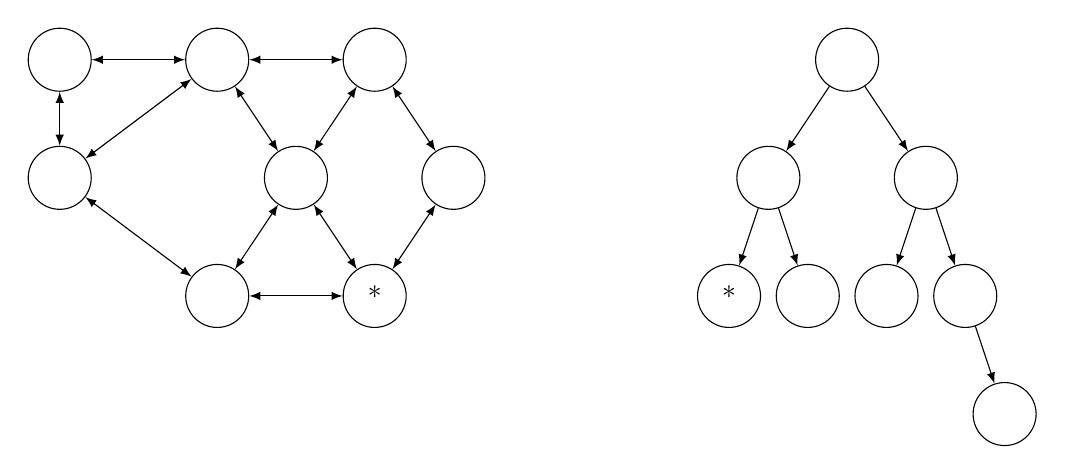
\begin{tikzpicture}
	%Network
	\node[draw, circle, minimum size=0.8cm] (0) at (0,0) {};
	\node[draw, circle, minimum size=0.8cm] (1) at (2,0) {};
	\node[draw, circle, minimum size=0.8cm] (2) at (4,0) {};
	\node[draw, circle, minimum size=0.8cm] (3) at (0,-1.5) {};
	\node[draw, circle, minimum size=0.8cm] (4) at (3,-1.5) {};
	\node[draw, circle, minimum size=0.8cm] (5) at (5,-1.5) {};
	\node[draw, circle, minimum size=0.8cm] (6) at (2,-3) {};
	\node[draw, circle, minimum size=0.8cm] (7) at (4,-3) {*};
	\draw[<->, >=latex] (0) -- (1);
	\draw[<->, >=latex] (0) -- (3);
	\draw[<->, >=latex] (1) -- (2);
	\draw[<->, >=latex] (1) -- (3);
	\draw[<->, >=latex] (1) -- (4);
	\draw[<->, >=latex] (2) -- (4);
	\draw[<->, >=latex] (2) -- (5);
	\draw[<->, >=latex] (3) -- (6);
	\draw[<->, >=latex] (4) -- (6);
	\draw[<->, >=latex] (4) -- (7);
	\draw[<->, >=latex] (5) -- (7);
	\draw[<->, >=latex] (6) -- (7);
	
	%Hierarchy
	\node[draw, circle, minimum size=0.8cm] (10) at (10,0) {};
	\node[draw, circle, minimum size=0.8cm] (11) at (9,-1.5) {};
	\node[draw, circle, minimum size=0.8cm] (12) at (11,-1.5) {};
	\node[draw, circle, minimum size=0.8cm] (13) at (8.5,-3) {*};
	\node[draw, circle, minimum size=0.8cm] (14) at (9.5,-3) {};
	\node[draw, circle, minimum size=0.8cm] (15) at (10.5,-3) {};
	\node[draw, circle, minimum size=0.8cm] (16) at (11.5,-3) {};
	\node[draw, circle, minimum size=0.8cm] (17) at (12,-4.5) {};
	\draw[->, >=latex] (10) -- (11);
	\draw[->, >=latex] (10) -- (12);
	\draw[->, >=latex] (11) -- (13);
	\draw[->, >=latex] (11) -- (14);
	\draw[->, >=latex] (12) -- (15);
	\draw[->, >=latex] (12) -- (16);
	\draw[->, >=latex] (16) -- (17);
\end{tikzpicture}
\caption{\label{Fig1}}
\end{center}
\end{figure}
8) Yet another way of saying the same thing is to say that anarchists are opposed to hierarchies. Because a hierarchy implies the resolution of differences by submission of one to another, it seems that hierarchy is inconsistent as a principle with free agreement. We might be willing to go along with hierarchical structures of voluntary organizations. That is a debatable point in principle, but in practice hierarchical organizations impose high costs of exit, that is, they are not in practice voluntary as a rule.\\
Structure is a necessity, to be sure, but anarchists urge the virtues of networks rather than hierarchies. (By the way, the so-called broadcast networks are actually hierarchies. That is what is wrong with them). Examples of the two forms are contrasted in the simple-minded diagram in Figure \ref{Fig1}. There are two important differences. In a network, the flow of information and influence is two-way, while in a hierarchy the flow of influence is downward ans the flow of information is either upward or downward but only ``through channels." It would appear that the hierarchy is a way to speed communication but (quite apart from the complications of communication between unequals) this is not so. Communication from the representative member of the group marked with an asterisk in the network to another arbitrarily chosen number will require an average of 1.86 connections or passages from one person to another. The comparable number for the asterisk-marked member in the hierarchy is exactly three. There are, of course, more lines of communication in the network -- eleven versus seven -- and interestingly enough, the product of the number of successive messages required times the number of channels required to keep the members in contact is about the same: 20.86 for the network, 21 for the hierarchy. This suggests to me that the two are about equally ``efficient" in some as yet undefined sense.\\
There is an old saying that human groups cannot be gotten together very easily, because whenever two groups join together one must be subjected to the other, and neither group will accept that willingly. This is true, so long, and only so long, as they are both organized in hierarchies. Figure \ref{Fig2} illustrates the point. The two hierarchies cannot be joined together without subjecting the boss of one or the other or both of them, as the one marked by the asterisk would be subordinated to the leader of the other group. It is not the rank-and-file who must be subordinated in order to join the two groups together, but the man who will make the decision whether to joint or not --- and he, of course, will resist subordination to the other hierarchy. Networks, however join readily and in a natural way, as illustrated in Figure \ref{Fig3}. Joining the two networks requires, at a minimum, only a link such as that between the two members marked with asterisks. This does not change the fundamental role of either of the members forming the link, though it increases their work load somewhat (this does not change the fundamental role of either of the members forming the link, though it increases their work load somewhat (this could be compensated by dropping one link, such as the links to the members marked with a \#) and it does not change the nature of either network. The ``law of nature" cited by Galbraith\footnote{Reference is to \emph{The New Industrial State}. Several editions are available.} and others, that ``orgranizations" always defend their autonomy, turns out to be oversimplified and misleading. True of course that the top men in hierarchies always protect their autonomy: others in hierarchies do no have any to protect. True, also, that hierarchies will not cooperate well, for that reason\footnote{Benjamin Ward, \emph{The Socialist Economy}, (New York; Random House, 1967) expands on this point. See ch.5.}. However, and without any sacrifice in the autonomy of either.\\
\begin{figure}[t]
\begin{center}
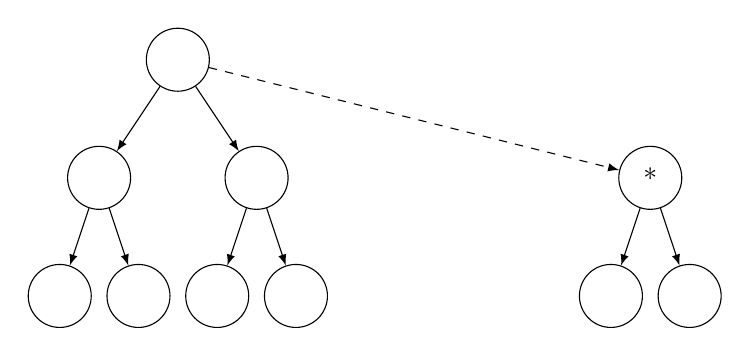
\begin{tikzpicture}
	\node[draw, circle, minimum size=0.8cm] (10) at (10,0) {};
	\node[draw, circle, minimum size=0.8cm] (11) at (9,-1.5) {};
	\node[draw, circle, minimum size=0.8cm] (12) at (11,-1.5) {};
	\node[draw, circle, minimum size=0.8cm] (13) at (8.5,-3) {};
	\node[draw, circle, minimum size=0.8cm] (14) at (9.5,-3) {};
	\node[draw, circle, minimum size=0.8cm] (15) at (10.5,-3) {};
	\node[draw, circle, minimum size=0.8cm] (16) at (11.5,-3) {};
	\draw[->, >=latex] (10) -- (11);
	\draw[->, >=latex] (10) -- (12);
	\draw[->, >=latex] (11) -- (13);
	\draw[->, >=latex] (11) -- (14);
	\draw[->, >=latex] (12) -- (15);
	\draw[->, >=latex] (12) -- (16);
	
	\node[draw, circle, minimum size=0.8cm] (20) at (16,-1.5) {*};
	\node[draw, circle, minimum size=0.8cm] (21) at (15.5,-3) {};
	\node[draw, circle, minimum size=0.8cm] (22) at (16.5,-3) {};
	\draw[->, >=latex] (20) -- (21);
	\draw[->, >=latex] (20) -- (22);
	
	\draw[->, >=latex, dashed] (10) -- (20);
	\end{tikzpicture}
\caption{\label{Fig2}}
\end{center}
\end{figure}

\begin{figure}[t]
\begin{center}
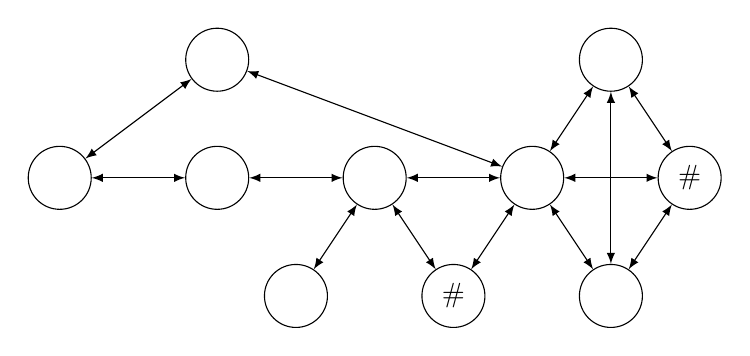
\begin{tikzpicture}
	\node[draw, circle, minimum size=0.8cm] (0) at (2,0) {};
	\node[draw, circle, minimum size=0.8cm] (1) at (7,0) {};
	\node[draw, circle, minimum size=0.8cm] (2) at (0,-1.5) {};
	\node[draw, circle, minimum size=0.8cm] (3) at (2,-1.5) {};
	\node[draw, circle, minimum size=0.8cm] (4) at (4,-1.5) {};
	\node[draw, circle, minimum size=0.8cm] (5) at (6,-1.5) {};
	\node[draw, circle, minimum size=0.8cm] (6) at (8,-1.5) {\#};
	\node[draw, circle, minimum size=0.8cm] (7) at (3,-3) {};
	\node[draw, circle, minimum size=0.8cm] (8) at (5,-3) {\#};
	\node[draw, circle, minimum size=0.8cm] (9) at (7,-3) {};
	\draw[<->, >=latex] (0) -- (2);
	\draw[<->, >=latex] (0) -- (5);
	\draw[<->, >=latex] (1) -- (5);
	\draw[<->, >=latex] (1) -- (6);
	\draw[<->, >=latex] (1) -- (9);
	\draw[<->, >=latex] (2) -- (3);
	\draw[<->, >=latex] (3) -- (4);
	\draw[<->, >=latex] (4) -- (5);
	\draw[<->, >=latex] (4) -- (7);
	\draw[<->, >=latex] (4) -- (8);
	\draw[<->, >=latex] (5) -- (6);
	\draw[<->, >=latex] (5) -- (8);
	\draw[<->, >=latex] (5) -- (9);
	\draw[<->, >=latex] (6) -- (9);
\end{tikzpicture}
\end{center}
\caption{\label{Fig3}}
\end{figure}

9) Fredrick C. Thayer's book, \emph{An End to Hierarchy! An End to Competition!}\footnote{(New York: Franklin Watts, 1973)} sounds like it might be an anarchist-communist tract. It isn't, and indeed the author's commitment to such authoritarian constructs as the MacDonald's hamburger chain, the U.S. Constitution and the National Security Council lend a surrealistic tone to the book's devotion to sweet consensus. Yet the book provides ample evidence of the productivity and importance of small groups, even within such organizations as those, and of the fact taht network structure is indispensable to every organization, however committed to formal hierarchy. Thayer's book is in the tradition of soft-headed or ``theory Y" management studies, as opposed to the hard-headed" or ``theory X" headbusters. However, Thayer's attitude to unions is pure paternalism.\\
Thayer finds that the ideal group size, in management studies, is five. One wonders if he might be a hidden Illuminatus\footnote{Reference is to \emph{Illuminatus!}, by R. Shea and R.A. Wilson, (New York, Dell, 1975) No flattery to the editor of this journal is intended by the mention, of course. Of course.}. A nice exercise for the brain is to read Thayer's book along with Robert Heinlein's \emph{The Moon is a Harsh Mistress}\footnote{(New York: Berkeley, 1968)}, if you can sneer at the militarism the two men share. But this leads us into science fiction, which is a horse of a different feather.\\

10) I think I have said enough, in this laundry list, to make my point. There is such a thing as anarchist ideology, even if it is mostly tacit in things we all take for granted. It is useful in that it helps us to communicate with others. That is a two-way street, and it is pretty certain that some of us don't want to communicate (we just want those others to listen) but it doesn't work that way. We can learn from social science, and even from business management, accounting and finance, if we approach those literatures critically. They can learn from us, maybe, but not unless we learn to communicate our ideas to them, in words, plain words, words that they are accustomed to using. For that we need explicit discussions of anarchist ideology, so that we can first understand one another.\\


\chapter{Out of the Closet with Jean-Paul Sartre}

The following is an excerpt from an interview with Jean-Paul Sartre by Michel Contat. The interview was first published in \emph{The New York Review} of August 7, 1975.\\

\noindent Q. After May 1968 you said to me: ``If one rereads all my books, one will realize that I have not changed profoundly, and that I have always remained an anarchist."\\

\noindent Sartre: That is very true. And it will be evident in the television broadcasts I ma preparing. Still, I have changed in the sense that I was an anarchist without knowing it when I wrote \emph{La Nausee}: I did not realize that I was writing there could have an anarchist interpretation; I was only the relation with the metaphysical idea of ``nausea," the metaphysical idea of existence. Then, by way of philosophy, I discovered the anarchist being in me. But when I discovered it I did not call it that, because today's anarchy no longer has anything to do with the anarchy of 1890.\\

\noindent Q. Actually, you never identified yourself with the so-called anarchist movement?\\

\noindent Sartre: Never. On the contrary, I was very far from it. But I have never accepted any power over me, and I have always thought that anarchy, which is to say a society without powers, must be brought about.

\chapter{Ode to Amazon Nation}
\chapterauthor{Arlene Meyers}

\begin{verbatim}
My mother was an Amazon
my daddy was a whore
I am a liberated woman
I don't struggle anymore

Mama fought the System
and confronted Daddy's power
Mamma made her revolution
it was her finest hour

Mom and Dad are old and tired now
living with memories
I spend my time in barrooms now
drinking gin and herbal teas

Amazon Nation has triumphed
and women run the show
we're politicians, cops and generals now
keeping our sisters in tow

The hand of the lady president
is the hand of a woman at war
the sex of the hand on the trigger
functions the same as before

          *         *
          
Oh sisters, what have we done
in asserting our womanly might?
we've castrated old Father Wrong
and deified good Mother Right

We looked for simple answers
avoiding struggle along with pain
not learning the lessons of his-tory
Sisters, we've lost again

          *         *

False consciousness divides us
and women on power trips
fragmented lives and egos
the fabric of sisterhood rips

Opportunists lust for power
others grab token reform
confused, we avoid the conflict
Sisterhood dies being born

The rule of State is Force and Fraud
theft and murder bloody its hand
the revolution founders in crisis
Sisters, where do we stand?

We need a woman's revolution
but change must begin in our heads
to mend our ravaged selfhood
with strong and vital new threads

All Power to the People
does not mean power to the few
let's cast our vanguards and dogma
and begin to struggle anew
\end{verbatim}


\chapter{The Role of Personal Differences in Organization}
\chapterauthor{Jim Bumpas}

Question: Why do anarchist organizations suffer disruption and many times suffer dissolution because of destructive personality clashes? This question is not dismissed by recalling that anarchist organizations aren't the only ones which suffer personality clashes.\\
I think I have some insight into at least two related causes. One cause is the social organization of people and things in our society which has concentrated great amounts of power, wealth and prestige into various centralized focuses. There is a whole spectrum from large, manipulative concentrations, down through mostly small, imitative concentrations which mostly provide practice for the ``real" competition in the large powerful organizations. These imitative organizations include especially student governments at schools and lodge and ``service" club organizations for working people.\\
These organizations, large and small, all offer the prizes of wealth, power and prestige in varying amounts, in addition to the enjoyment of comradeship and group effort which may be found in many organizations. In fact, these material rewards are distinct from, and not at all related to the purposes of the collective work of most organizations like political parties and non-profit organizations.\\
Another cause is the destructive social conditioning we all suffer which makes us want to scratch, bite and claw our way to the top of any of these organizations. This conditioning adequately serves the control and domination purposes of establishment organizations. The resources they control and the coercive machinery of the state are available to them for protection. So the competitors for position are forced to conform to the dog-eat-dog way of life. Slight personal differences basic to our individuality are struck upon and exaggerated both to justify one's fight against someone in his way and to serve as a tool to beat the competitor down.\\
Anarchist organizations control no such set of socially-sanctioned prizes. The reward of collective work in such organizations is just that collective work and the comraderie of closeness to persons of similar social perspectives.\\
However, all of us enter anarchist organizations carrying various amounts of baggage containing this ``scratch, bite, and claw" conditioning. We are all affected somewhat by the desire for material rewards. These two factors produce disruption and destruction to anarchist organizations.\\
We practice in our organizations many of the same destructive relationships found in the society we desire to alter. We strike upon some real or fancied minor difference in personality or approach and try to elevate it into a grand ideological distinction. This leads one to try to purge the other, or bend the other to conform to one's criticism. Or, failing all that, one can split the group and lead your followers out.\\
Even in a group whose members share similar or perhaps the same perspectives --- even when method and practice are exact --- a minor shift in emphasis between two or more persons can give rise to the destructive abandoning of the purposes of the group's collective work. One person begins to play down media/theater type actions and stresses the importance of concentrating all activity on contacting people where they work, live or play in order to provide organizational tools for the expression of and achieving their desires. Another downplays such activity and stresses the consciousness-altering value of shocking media/theater actions. Another plays down both and stresses the need for direct, violent action against persons and institutions identified as oppressive.\\
These differences arise mostly because of differences in individual personality and in personal evaluations of current circumstances, both of society in general and the organization and its individual members. But instead of mutual recognition of each other's mutual dignity and personality, and instead of attempting to analyze clearly personal interrelationships and current circumstances, many times these differences are elevated into grand ideological distinctions. Instead of discussing social conditions and organizational resources in order to adopt the tactics which most fit present capacities for action, our mutual perspectives are abandoned --- and real people are abandoned, too --- in order to develop, preserve and protect the rarified ideological purity of one person or another. The exaggerated ideological/personal differences become so important that group effort suffers and withers away. The group splits or shatters and constructive work ceases until everyone begins again, almost from scratch in some cases. Sometimes, constructive group work only begins to grow again as a result of another split in another group. Old Splittees  join new splittees in common aversion to the splittees of the other ``side."\\
In anarchist organizations there is no position equivalent to chairman of the central committee or president. Nor are there big salaries given as plums to the victors in the struggle between personalities. So the groups divide, or they fail to collaborate or affiliate in solidarity for the common project. Each little groupuscule isolates itself from the other and creates for itself much of the alienation felt by anarchists toward some other anarchists.\\
I'm convinced it's a mistake and a violation of our perspectives to try to correct the problem by creating some ``anarchist" equivalent to the hierarchy or salaries of the authoritarians. But we cannot ignore the problem. Perhaps clear analysis of some of the causes for disruption in our work will allow us to minimize the destruction caused by these personality clashes. Comparison of our forms organization to those hierarchical forms found in society around us will aid us in this analysis. Why do we differ from them? Why must authoritarians maintain hierarchy and how does it further their goals? Can we organize society without hierarchy and the motivations which impel people to work within authoritarian forms?\\
It appears to me that we must show some spectacular success in organizing ourselves along anti-authoritarian lines before we can make a significant advance against the popular authoritarian assumption that nothing gets done unless someone orders others to do it.


\chapter{The Secret Teachings of George Washington}
\chapterauthor{General Strike}

George puffed the reefer and passed it to Tom Jefferson, who was involved in an act of coitus with Discordia, the black ``slave girl" (so thought the unitiatied) (Discordia Jefferson, incidentally enough, was the great-great-great grandmother of Robin Jefferson of modern-day Fucking Communist Conspiracy fame.)\\
Washington spoke these words in reply to Jefferson's contention that the proposed Constitution would lead to tyranny (which had been Franklin's response, at first): ``No. Because of the 13\cent stamp."\\
\textsc{Jeff:} The 13\cent stamp?\\
\textsc{Geo:} Yeah. I give the Constitution 200 years. after that will be the 13\cent stamp.\\
\textsc{Ben:} That's why we have to see that the Federal Government maintains a monopoly on first-class postal business. Dig?\\
\textsc{Geo:} In 1976 --- on New Year's Day --- the Postal Service (which is what it will then be called) issues the 13\cent stamp --- as an omen of the end, as an endorsement of the Indian hemp plant, a commemoration of the 13 colonies who defied the Crown, as a call to revolution, and as an ``inflationary measure of economic necessity" or some similar fiscal responsibility doubletalk --- as if an institution traditionally devoted to losing money needs to worry about inflation!\\
\textsc{Ben:} Right. And you see, the Illuminati will have engineered the most drastic inflationary spiral in the nation's history during '75 solely to enable the Postal Service to credibly raise the price of mailing a first-class letter to 13\cent.\\
\textsc{Geo:} And all first-class mail will thereafter be transported by air, too. Because, in reality, the 13\cent stamp will be a sign --- an omen of the end, an endorsement of the Indian hemp plant, a commemoration of the 13 colonies who defied the crown...\\
\textsc{Discordia:} And a call to Revolution.
\textsc{Ben:} And millions upon millions of these stamps will be on letters which will be in the air over the continent every day.\\
\textsc{Geo:} So Illuminati agents can point out that there are ``signs in the sky."\\
\textsc{Discordia:} That way we prepare the Bible freaks for the change. And not only that. George, tell him about women's liberation angle.\\
``Let me tell that part," said Ben Franklin, expelling a large cloud of smoke (being as he was into women's liberation vicariously as a closet case drag queen, during odd moments between flying kites in lightning storms and printing them \emph{Saturday Evening Post}. ``One of the secrets to which we Rosicrucians are privy is that the number 13 signifies death and resurrection. That is why there were 13 people at the Last Supper. But they were all men, so..."\\
And so they spoke long into the night about secret things, many of which cannot be revealed until the time is ripe.

\chapter{The Ether Vibrates}
\vspace{-1cm}
\emph{Letters from Readers}\\

\noindent \textsc{Chicago, Illinois:}\\

\begin{flushright} 
\begin{tabular}{l p{8cm}}
1931 & Nel forte Braschi di Roma l'anarchico Michele Schirru viene fucilato, perche scoperto mentre attuava un attentato contro Mussolini
\end{tabular}

In the Year of the BOMB --- XXX\\ \end{flushright}

\noindent \emph{no governoR.S.}:
\indent I particularly liked Anton's bitt for ``FREE LOVE... AND ALL THAT". I hope it gets widely copied.... In regard to McNamara's \emph{Greedy Gurus}, the ``Father" is D\emph{e}vine, not Divine.... Regarding ``... The Necessity for Pacifism", there shd be, not a comma, but a period separating \emph{practice} and \emph{War} (p. [26], line [6] from [top]). On p. [29], line [3 from bottom], \emph{thanks} not \emph{`thaks}.' And in the 2nd line of the concluding CAVEAT: \emph{auti-authority}, not \emph{`anti-aughority'}\\
In ``Doing Anarchis Yourself" you seem to come out for the inheritance of acquired characteristics where you write: ``The anarchist movement, little more than a century old, represents a beginning effort by some members of our species to erase that neolithic authoritarian mind-set programming and try to think about human problems in a new way".\\
More important, perhaps, is the nature of the group. I do not regard myself as more important than the group I may be part of. The group is composed of myself and others in interaction. To regard myself as more important might directly of indirectly connote some carelessness toward, or contempt for, others in the group. Not even Stirner, in his Unions of Egoists, wd have so cavalier and attitude toward others with whom he might be in association (altho Stirner incorrectly conceived an inhenrent conflict between the needs of the Ego --- if he meant Egos other than his own --- and the nature of association). A group, particularly an an-archist group, exists in order to satisfy a need for revolution. Such a group shd not exist merely ``to satisfy the needs of individual members". If that were the case, the group wd tend to become a psychotherapy affair: a waste of time. In a group, as in social intercourse generally, one shd seek a balance between the egoistic and altruistic interests of individuals. And in a balanced relationship, the group might have equality with its members.\\
Your theory of the group cd easily lead to Arlene Meyers' criticism of an-archism as ``an anti-social movement".\\
Another thing; I think anti-Authoritarian groups can be as well defined, at least on paper, as Authoritarian groups. Not to be as well defined can be tantamount to not knowing who or what we are or what we are about. SRAF has principles, but I do not think that the schedule of principles makes it less an-archist. Since I made a contribution to those principles, I think SRAF is \emph{more} an-archist because of them. The trouble was that entities like Tyrone, WAP, etc., participated, seemingly as members, when they did not understand or accept (or know of?) the anti-archic waters. I do not reprove the openness by which this happened, but it shd be obvious that if we are more available for penetration by vigorous, eccentric authoritarian elements, then we will have a much harder time getting ourselves together to do anything, as compared with the efficiency of authoritarians to get themselves together to smash us or to compute society like a prison.\\
I am not one of those hostile to all forms of leadership on principle. If I were, I might have opposed your initiative from which the nameless anarchist horde got started. Of course, I oppose all the leadership, out of hand and sight unseen, that needs coercion, hierarchy, or which expresses racism, sexism. But as regards groups such as you and Arlene discuss, the ideal shd be that of a balanced distribution of the functions of leadership. Failing that, the leadership may be useful or valuable as long as it is correct. (The leadership of organizing individuals in limited economic situations is offered or defended as a principle of organization by some aligned with the Warren tendency of individualist an-archism\footnote{This is not more, Bob, than what you do, when as non-governor, you lay down the rules, format and frequency for participating in \emph{No Governor}.}.\\
A. Meyers, discussing the an-archist movement on p. [15], writes: ``our heads are really the first battleground where we initiate the struggle against the state". And in your article, you write: ``One new thing that has to be learned and is rarely fully appreciate is the role of the individual in anarchism." The role of the individual in an-archism is to initiate the struggle against the State, in h/er/is own head, by renouncing citizenship. By defining ourselves to ourselves and to others as STATELESS PERSONS OF THE WORLD, \emph{and shouting it from the housetops}, as it were, we begin to break some new ground against democracy and patriotism. Theories that were well enf adapted to fighting the autocracy of the Czars may be lacking in strategic emfases in situasions where the citizen is h/er/is own worst enemy merely because s/he thinks of self as a citizen, and where the worst despotisms sell themselves to the public as ``democratic". If we can make an-archism clear to ourselves as STATELESS PERSONS OF THE WORLD, then we can make it clear to others. We certainly DO NOT make an-archism clear to the average Jo(e) if s/he thinks we are somebody `just like h/im/er'. There shd be an important and essential difference between us and this average Jo(e) and just letting Jo(e) know that we do not belong to h/is/er nuclear club (The State) can have more propaganda value than all the an-archist lit printed since 1965. And some of the solutions we are seeking may flow from our own self-concept, once we put it bluntly, relevantly and correctly to our personal selves an to others.\\
Those who renounce citizenship may not be able to carry a passport to an international an-archist congress. (As it is now those go who have the money or transportation.) Until an-archists, as a movement, can get together on it, there is no alternative but for the conscientious an-archist to declare for Statelessness and disqualify Self for the paper that might deliver h/er/im to an an-archist congress abroad. But if, say, 63 percent of the known an-archists sort themselves out by lottery into those who renounce citizenship and those who might travel on the State's paper, there wd be some available to travel that way. As new people renewed or enlarged the ranks of those organized for STATELESSNESS, their lot wd be cast, periodically, with the moiety that did not luck-out of citizenship: they wd have the same chance of lucking out as all those who did not luck-out of citizenship (formally) in the previous lottery. A renunciation of citizenship, is of course, irreversible (how can an an-archist become, let alone re-become, a citizen?) and the pool of an-archists who have not formally renounced citizenship is continually giving up members to explicit STATELESSNESS. This scheme is not meant to provide a loophole to an-archists who have not explicitly renounced citizenship so that they may think they are justified in voting against GoldwaterWallaceReaganApeshit or voting for WAPLibertarianPartyCitizenshit. If if has the faintest possibility of being interpreted that way, then it shd be junked, discarded without any further consideration. The idea is not to weaken an-archism but to strengthen it. If the scheme can be exploited as to support political participation, then the infra-structure of an-archy is too compromised and subverted by Democracy and Liberalism. It wd be better for all who understand an-archism correctly to unreservedly declare for STATELESSNESS and forego any tactical advantage that the lottery might afford the international movement.\\
At any rate, a given lottery pool shd come to term at the end of 9 or 14 years which means that everybody in the pool wd declare for STATELESSNESS and a new 9 yr. pool started with newcomers. (Better, terms of different lengths --- 9 or 14 --- cd be assigned to joiners. This wd ensure a continuity).\\
It is too much like a disgrace that International An-archist congresses are helf with people who arrived on passports. If these Congresses concluded with most or all of those on passport burning them and declaring themselves STATELESS, then the Congresses might serve as a useful demonstration of anti-patriotism, anti-nationalism, an-archism \& human solidarity. I do not say that we shd get rid of such Congresses, questionable as they may be. This is not an attack on the an-archist movement: we need all that we have. But I do say that International An-archist Congresses shd be called where participants from abroad do NOT have tourist card, visa, permit, passport or other politically certified travel papers. Whether such an International Congress cd reach a `quorum' (whatever that might mean for an anti-parliamentary gathering) remains to be explored. But an-archist activity, including ``going limp" when made \& held captive, at check points or border crossings wd practically be assured. A chance to do something about the main impediment to human solidarity. With an an-archist interpretation that \emph{ATTACKS} the worldcitizen-worldgovernement terminology.\\
And there is no reason why we shd not call such International Congresses in places like Gulai-Polye, Changsha, or Chicago (an-archists have beend forbidden by law to enter USA since 1903). We might have as much success getting together without passports in those places as anywhere else.\\
It goes without saying that anarchists, like Jesus, shd be born bastards. The an-archist who has a child who is not bastard has something to explain --- mainly to the child. But the point here is that there shd be a way for a child to be born without automatically  being tainted with citizenship and nationalism: the democratic imposition of identity. Is the immaculate conception possible? At any rate we shd try, and publish the places and ways a child might at least come into the world STATELESS. If the ungrateful brat wants to rebel against its parents and kiss the feet of Grace Kelley, live among the bogey men of Haiti or wallow in the despotism of Israel or USSR, it will, unfortunately, probably have such chance before we can turn the world upside down and make such options available.\\
Arlene Meyers, in her ``The Anarchist Movement --- Dead of Alive?" suggests that a ``lack of direction" contributed to the demise of a Chicago an-archist group. I wd suggest also that that group's failure to meet a challenge of patriotism in regard to a 5th of July parade (Evanston, ILL), also contributed to the group's demise --- internal disintegration --- because a dishonest maneuver was resorted to in order to blunt part of the attack that might have been made on patriotism. The dishonest maneuver was fount out, and the expose, limited as it was, unglued some relationships.\\
In other words, we trick ourselves when we treat patriotism flippantly, condescendingly, lightly, when we treat it as not as important as, say, wage struggles. It is much more serious than wages \& hours struggles except when strikes occur in war industry. At that point they become the same problem, because the workers shd not be trying to improve their wages \& hours position, they shd be trying to destroy it utterly and irrevocably insofar as it is connected to war work. And this workers' attack on military employments shd be delivered with attacks on patriotism. Patriotism is the most dangerous religion around.\\
Near the top of page [12], Arlene speaks of ``integrating our politics? with our daily lives". Since an-archists, as ANTI-political animals, do NOT have `politics', it follows that it is our ANTI-POLITICS that we shd be intergrating with our daily lives.\\
Jim Bumpas, in 3 places in his ``Should We Cooperate?" refers to the ``corporate establishment" which dominates our culture and society. I think ``corporate establishment" is a misleading piece of new left rhetoric, because it is the people who lend money, especially those who lend money to Governments who orient the status quo and draw its basic outlines. In this lite, ``corporta establishment" is more like a cover-up for the WASP-Jewish money what runs it than anything else.\\
Bumpas says: ``It is to our advantage to tip the status quo out of balance". And he says that, by so doing, ``we will not be swallowed up whole as the Bolsheviks swallowed anarchists in Russia" even while the CP in Portugal is swallowing up everything. We shd recognize that the present balance of the status quo probably protects us more that it threatens us, both from ``Left"-authoritarians and the Rightracistreactionaries. The present balance of the status quo is probably the best protection going for most Marxists, because the sect that gets the Power will probably smash all the rest, much like they are trying to dow, and are doing in Portugal.\\
We shd not be trying to ``tip the balance" of the status quo. We shd be trying to collapse it utterly: no authoritarian arrangement for either the political left or the political right to work thru.\\
This is not an argument against cooperation since I probably do more of it (with \emph{Marxists}) than most an-anrchists who read this. The advantage of cooperation is that it gives \emph{Marxists} a chance to disabuse themselves of their stereotypes (frequently, stereotypes indistinguishable from the bourgeois stereotypes). Those of us who have been \emph{Marxists} know what that means. And those of us who understand the difficulties with black-white stereotyping may understand the size of this job.

\par\begin{flushright}
\begin{tabular}{l}
Joffre Stewart\\advocate of the \emph{ANTI}-Christ\\6114 S. May Street\\Chicago, Illinois 60621 
\end{tabular} 
\end{flushright}


\chapter{The Frying Pan}
\vspace{-1cm}
\emph{Reviews of Libertarian Publications Recently Received}\\

\noindent\textsc{Against the Wall.} A libertarian magazine. Volume 4 Number 5 is largely book reviews, including \emph{A Gang of Pecksniffs} by H.L. Mencken, \emph{Against Our Will} by Susan Brownmiller and \emph{The Air Force Mafia} by Peter N. James. This issue costs 50 cents, but future issues will be 75 cents. Against the Wall, P.O. Box 444, Westfield New Jersey 07091.\\

\noindent\textsc{Black Star.} An Anarchist Review. A publication of the Social Revolutionary Anarchist Federation. Continues to improve dramatically with each issue, as the continent-spanning collective that edits and publishes it gains in experience. For us, highlights of Issue Number 3 were ``Homo Economicus" by Glenn Meredith, on the way capitalism has conditioned people to feel artificial needs; ``Quality or Quantity" by Jersey, on anarchist agitation among the people right around you; and ``Towards an American Anarchism" by Irving Levitas on 19th-century grassroots religious movements whose ideas tended toward anarchism. There's much more (32 pages) to make the 25-cent cover price a bargain. Subs are six issues for \$3, \$10 for institutions, free to prisoners. Black Star, Box 92--246, Milwaukee, Wisconsin 53202.\\

\noindent\textsc{Equality.} A Libertarian Review. A one-sheet publication usually devoted to profiles of lesser-known anarchists, together with information on their published writings and on writings about them. As these keep coming out, a collection of \emph{Equality} portraits will become more and more useful. Volume I, Number 1 is devoted to Jan Waclaw Machajski, Polish-Russian social theorist and revolutionary. Number 2, Voltarine deClayre, American anarchist writer. Number 3, a very complete and up-to-date bibliography on Bakunin. Number 5, Rudolf Rocker, editor and labor organizer. Number 7, Robert Reitzel, 19th century German-American anarchist. From The Kropotkin Society, Post Office Box 2418, Evansville, Indiana 47714.\\

\noindent\textsc{Libero International.} Published in Japan, in just three issues this anarchist magazine has become the indispensable guide to the libertarian left in Asia. Issue number 3, November, 1975, includes a profile of the Hong Kong 70s Front, an anti-authoritarian socialist group; a continuation of the history of hte Chinese anarchist May 4th movement; the first installment of a history of the Korean anarchist movement; the story of an effort by Japanese farmers to resist eviction for an airport to be built on their land; much more. Published quarterly. \$3 for six issues, single copies 50 cents; send money orders or cash, not personal checks. Libero Internation c/o CIRA-Nippon SIC, C.P.O. Box 1065, Kobe, Japan 650--91.\\

\noindent\textsc{The Match!} Long-established tabloid newspaper out of Tucson, Arizona. Articles are tough-talking and frequently take out after others on the libertarian left as well as against anarchism's customary enemies. The April-May, 1976 issue, Volume 6 Number 11 is full of good reading: articles on the swine flue scare, gun control, individualism and despotism, materialism and vengeance as an anarchist principle. A column called ``Random Shots" by editor Fred Woodworth sets the lively polemical tone for the whole paper. Sample copy 15 cents, 12-issue subscription for \$3. The Match! P.O. Box 3488, Tucson, Arizona 85722.\\

\noindent\textsc{Open Road.} A stunningly handsome 32-page newspaper from a collective in Vancouver, British Columbia. Describes itself as ``designed to reflect the spectrum of international anarchist and anti-authoritarian Left activities and to provide reports and analysis of popular struggles and social problems. It is not the organ of a political organization." Name comes from Emma Goldman's original name for her magazine, which was eventually called \emph{Mother Earth}. First issue includes articles on Greepeace, resistance in Chile, protest against Trident submarines, the Symbionese Liberation Army, Kansas City Yippie convention, the Movement ethic, Holly Near, Martin Sostre, the American Indian Movement, the late Phil Ochs and women's labor organizing. The cover price is 60 cents, but the publishers say they have no subscription rates and depend on people's donations. It's very impressive and worth whatever you send them. The Open Road, Box 6135, Station G, Vancouver, B.C., Canada.\\

\noindent\textsc{Solidarity Newsletter.} A handsome, large-format four-page publication. News, reviews and letters for a libertarian-left audience. Number 12 presents a review of \emph{The Dispossessed} by Ursula K. Leguin, a science fiction novel dealing seriously and in detail with an anarchist society of the far future; an article on an attempt at tenant control in some New York City apartment buildings; an announcement that \emph{Solidarity Newsletter} may merge with a publication called \emph{Synthesis}. 15 cents a copy, the issues for \$1.50. Philadelphia Solidarity, Box 13011, Philadelphia, Pennsylvania 19101.\\

\noindent\textsc{Southern Libertarian Review.} A magazine of the libertarian right, which is for private enterprise, takes some inspiration from Ayn Rand and is against the government up to a difficult-to-determine point. The August 1976 issue, Volume 2, Number 11 includes ``The Canal Issue" by E. Scott Royce, ``A libertarian Nation?" about an enclave in Jamaica by Adam Starchild, ``William Jennings Bryan" by Robert Brakeman, and ``In Defense of the Non-Aggression Principle" by Jarret B. Wollstein. SLR, c/o E. Scott Royce, 1236 S. Taylor Street \# A, Arlington, Virginia 22204. 12 issues for \$6.\\

\noindent\textsc{Sweet Gherkins from the Dill Pickle Press.} The January 24, 1976 issue includes an analysis of fascism in George Wallace's presidential campaign, as well as brief excerpts from the works of Rabindranath Tagore, Stuart Chase, William J. Fishman, Donald Ogden Stuart, W.C. Fields and Paul Goodman. Two of the most interesting items in the May 24 issue were a statement by Charles S. Pierce on morality and one by Margaret Macdonald on political language. Subscription 10 issues for \$1, single copy 10 cents. 


\chapter{The Dialectic of Morality}
\chapterauthor{Josh the Dill}

Why are we forever patting ourselves on the back because we practice virtue and pursue ideals? Why are we condemning each other all the time for being immoral? Because, we say, our efforts at morality, virtue and idealism have raised us above the level of the beasts. Some justification! Who, when he or she really considers the matter, would really want to be above the level of the beasts, and why? Beast do not destroy their own environment, do not massacre millions of their own species, do not practice sacrifice of their own kind to propitiate spooks. The human race likes the idea of feeling superior to animals because it is on an ego trip. We vaunt our civilization, the extent to which we have created defenses against the sort of suffering animals must endure. Bur our ideals and values have produced their opposites. If there were no goodness, there would be no evil. No law and order, no crime. Every figure calls up a ground, every black implies a white. The distinctions between black and white and the rest are necessary, but so is recognition of fundamental one-ness. This point applies to violence and nonviolence. Making nonviolence a moral absolute will provoke violence. Violence, in turn, generates nonviolence as a response. Martin Luther King's nonviolent march from Selma to Montgolery was protected by Federal paratroops.

\newpage
\blockquote{``Utopia must spring in the private bosom before it can flower in civic virtue, inner reforms leading naturally to outer ones. A man who has reformed himself will reform thousands.
\par\begin{flushright} --- Paramahansa Yogananda, \emph{Autobiography of a Yogi}\end{flushright}
}

\end{document}


















